\documentclass[11pt]{article}

%\usepackage[left=0.2cm, right=0.5cm]{geometry}
\usepackage{amsmath}
\usepackage{amssymb}
\usepackage{graphicx}
\usepackage{multirow}
\usepackage{array}
\usepackage{pgf}
\usepackage{pgfpages}
\usepackage{lipsum}
\usepackage{xcolor,colortbl}
%\usepackage[a4paper,margin=1in,footskip=0.25in]{geometry}
\usepackage{comment}
\usepackage{multirow}
\usepackage[a4paper,footskip=0.2cm,margin=0.5cm,left=0.4cm, right=0.4cm]{geometry}
\pagestyle{empty}
%\setlength{\voffset}{-0.5in}
%\setlength{\textheight}{710pt}
\usepackage{array}
\usepackage[T1]{fontenc}
\usepackage{lmodern}
%\renewcommand{\familydefault}{tgtermes}
\usepackage{color}
%\title{}
%\author{CIS 160 Fall 2014}
%\date{19 September 2014}


\pgfpagesdeclarelayout{boxed}
{
  \edef\pgfpageoptionborder{0pt}
}
{
  \pgfpagesphysicalpageoptions
  {%
    logical pages=1,%
  }
  \pgfpageslogicalpageoptions{1}
  {
    border code=\pgfsetlinewidth{2pt}\pgfstroke,%
    border shrink=\pgfpageoptionborder,%
    resized width=.98\pgfphysicalwidth,%
    resized height=.98\pgfphysicalheight,%
    center=\pgfpoint{.5\pgfphysicalwidth}{.5\pgfphysicalheight}%
  }%
}

\pgfpagesuselayout{boxed}



\begin{document}
%\maketitle

%\setlength{\parindent}{0pt}

\begin{center}
%\begin{tabular}{ |p{3.5cm}||p{9cm}||p{3.5cm}|  }
%\begin{tabular}{ |p{0.27\textwidth}||p{0.27\textwidth}||p{0.27\textwidth}|  }
%\begin{tabular}{ |m{0.28\textwidth}||m{0.28\textwidth}||m{0.28\textwidth}|  }
%\begin{tabular}{ |c{0.27\textwidth}||c{0.27\textwidth}||c{0.27\textwidth}|  }

 %\begin{tabular}{|m{0.28\textwidth}||m{0.28\textwidth}||m{0.28\textwidth}| }
 
 \begin{tabular}{| >{\centering\arraybackslash}m{0.28\textwidth} | m{0.28\textwidth} | >{\centering\arraybackslash}m{0.28\textwidth} |}

 \hline
    \begin{minipage}{.25\textwidth}
	\centering
      
\includegraphics[width=3cm, height=10mm]{-logo-.png}
    \end{minipage}   
    & \vspace{0.1cm} \textbf{Nome misura}: -nome!misura-  \newline \textbf{Strumentazione}: -strumentazione-
 \newline \textbf{Data e ora}: -data!ora- \vspace{0.1cm} &  {\large\textbf{Punto di misura: -punto!misura-}} \\
 \hline
\end{tabular}
\end{center}

\begin{figure}[!htb]
   \begin{minipage}{0.6\textwidth}
     \centering
     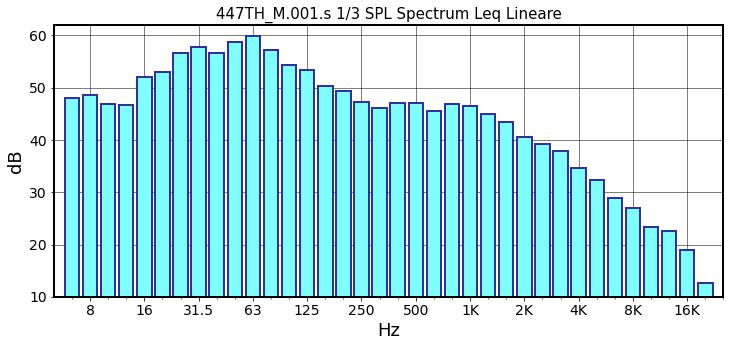
\includegraphics[width=1.\textwidth]{-SPL!plot-}
%     \caption{Interpolation for Data 1}\label{Fig:Data1}

	\begin{center}
	\begin{tabular}{|c || c |} 
	 \hline
	 L1: -L1- dBA & L5: -L5- dBA \\ %[0.5ex] 
	 \hline
	L10: -L10- dBA & L50: -L50- dBA \\ 
	 \hline
	L90: -L90- dBA & L95: -L95- dBA \\ %[1ex] 
	\hline
	\end{tabular}
	\end{center}


	\end{minipage}\hfill
     \begin{minipage}{0.4\textwidth}
	\begin{center}
%	\begin{tabular}{ |p{0.6\textwidth}|} 
%	 \hline
%	 Note: \newline \newline \\ 
%	 \hline
%	\end{tabular}
%	 \centering
%     \includegraphics[width=0.3\textwidth]{1697533982792.jpg}
     	\begin{tabular}{ |p{0.6\textwidth}|} 
	 \hline
%	 \hline
	 \textbf{Note}: \newline -note- \\ 
	 \hline
    \begin{minipage}{.5\textwidth}
    \vspace{0.3cm}
    \hspace{0.8cm}
	\centering
%      \includegraphics[width=0.7\textwidth, height=3cm]{1697533982792.jpg}
      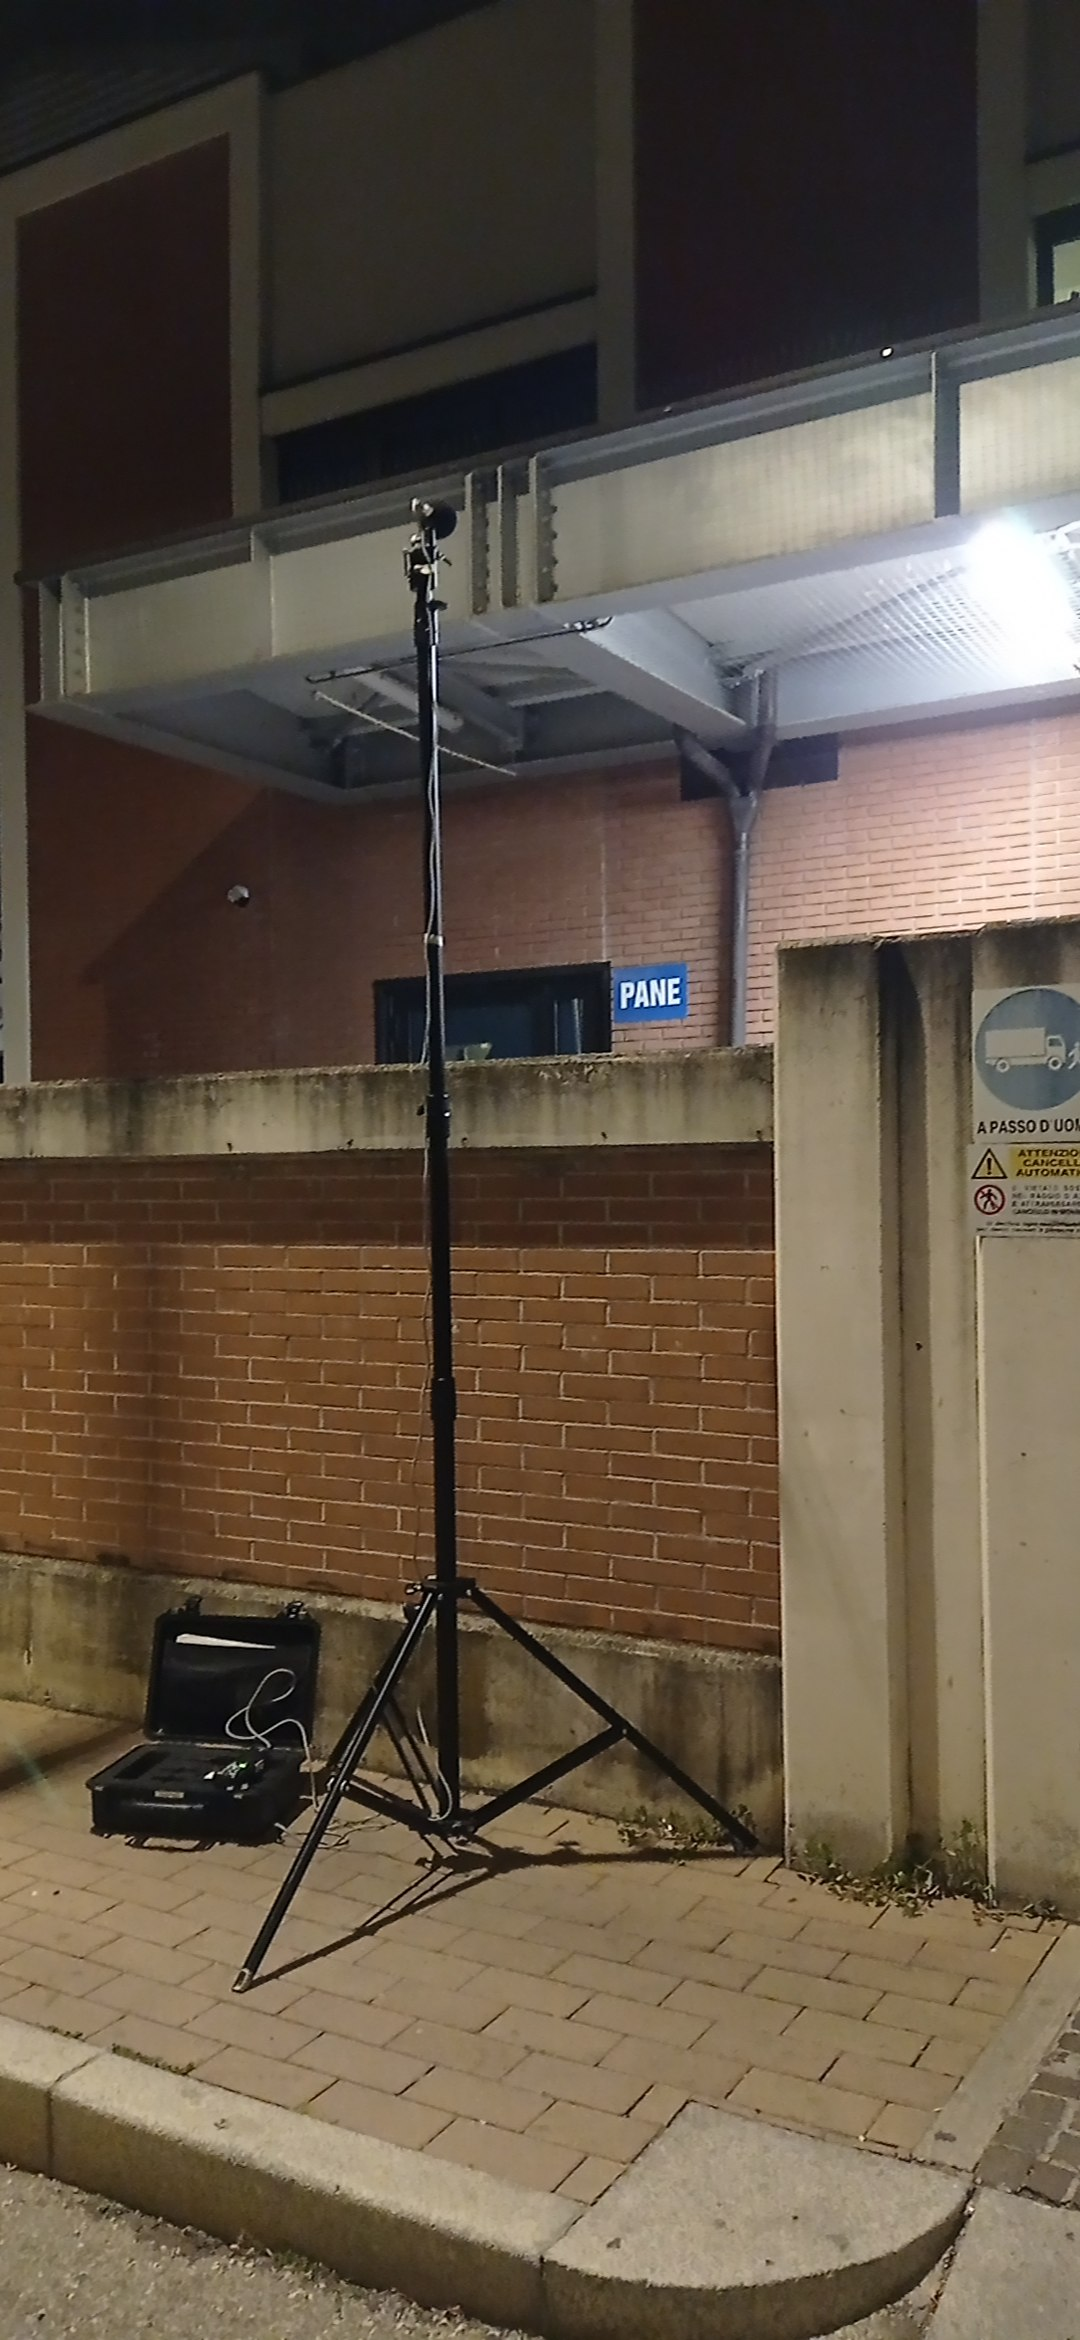
\includegraphics[height=5cm]{-foto-V.jpg}
     \vspace{0.3cm}
        \end{minipage}	 \\
        	
	\hline\hline \\ %[0.1cm]
 %\cellcolor{yellow}  \hfil   \textbf{LAeq: -LAeq- dBA} \\ %[0.3cm]
%  \cellcolor{yellow}  \textbf{LAeq: -LAeq- dBA} \\ %[0.3cm]

	\Large{\textbf{LAeq: -LAeq- dBA}} \\ %[0.3cm]
	\hline 
	\end{tabular}
	\end{center}


   \end{minipage}
\end{figure}

%----------------------------------time history-----------------------------

\begin{figure}[!htb]
     \begin{centering}
     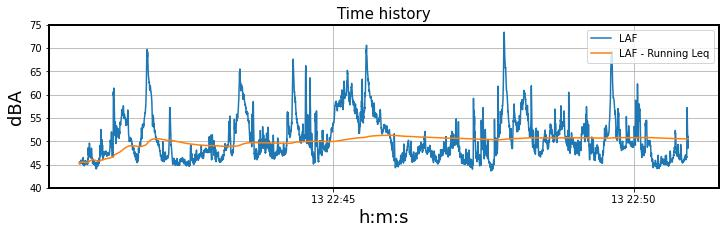
\includegraphics[width=0.94\textwidth]{-time!history!plot-}%\hfil
     \end{centering}
%     \caption{Interpolation for Data 1}\label{Fig:Data1}
\end{figure}

%-------------------------------mascherature------------------------------
\vspace{-0.3cm}

\centering
%\begin{tabular}{ |p{3.5cm}||p{3.5cm}|p{3.5cm}|p{3.5cm}|  }
%\begin{tabular}{ |p{0.21\textwidth}|p{0.21\textwidth}|p{0.21\textwidth}|p{0.21\textwidth}|  }

\begin{tabular}{| >{\centering\arraybackslash}m{0.21\textwidth} |  >{\centering\arraybackslash}m{0.21\textwidth} |  >{\centering\arraybackslash}m{0.21\textwidth} |  >{\centering\arraybackslash}m{0.21\textwidth} |}

 \hline
 \multicolumn{3}{|c|}{\textbf{Tabella mascherature}} \\
 \hline
\textbf{Nome}&  \textbf{Durata} &\textbf{Leq}\\
 \hline
Totale & -durata!tot- &  -LAeq!tot- dBA\\
 \hline
Non Mascherato & -durata!non!mask- &  -LAeq!non!mask- dBA\\
 \hline
Mascherato & -durata!mask- & -LAeq!mask- dBA\\
 \hline
\end{tabular}

%\vspace*{-2cm}
%---------------------------------spettro minimi--------------------------------

\vspace{-0.2cm}

\begin{figure}[!htb]
\centering
     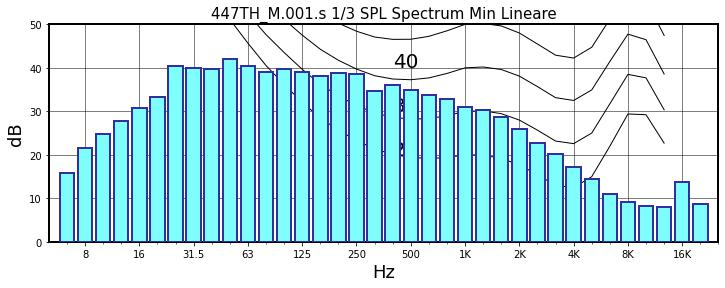
\includegraphics[width=0.93\textwidth]{-SPL!min!plot-}%\hfil
%     \caption{Interpolation for Data 1}\label{Fig:Data1}
\end{figure}

\end{document}